\chapter{Quantum Circuits} \label{chap:circuits}
Multiple qubits in combination with quantum gates can be arranged to a quantum circuit.
Initially, each qubit is set to the state $\ket{0}$ and subsequently transformed through the application of quantum gates.
Apart from qubits and quantum gates, a quantum circuit also consists of classical bits and measurements.
Qubits can be measured at any point in the circuit.
Upon measurement, the state of a qubit collapses to either $\ket{1}$ or $\ket{0}$, and the result of the measurement is stored in one of the classical bits.
Figure \ref{fig:example_quantum_circuit} shows an example for a simple quantum circuit.
The aim of this chapter is to fully understand and describe this circuit.
\begin{figure}[H]
	\centering
	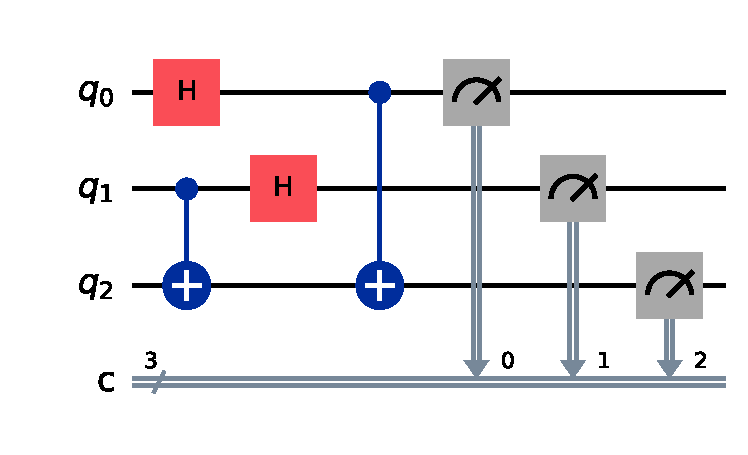
\includegraphics[width=0.5\linewidth]{figures/example_quantum_circuit.pdf}
	\caption{This is an example of a simple quantum circuit. There are three qubits $\{q_0,q_1,q_2\}$, whose states are transformed by two single-qubit gates—Hadamard gates (H) in this case—and two multi-qubit gates, specifically controlled-X (CX) gates. At the end, each qubit is measured, and the result is stored in three classical bits. This visualization of a quantum circuit was generated using Qiskit \cite{qiskit2024}. The source code for this figure can be found in Listing \ref{lst:example_circuit_source}}
	\label{fig:example_quantum_circuit}
\end{figure}
\section{Quantum gates}
	A quantum gate in a quantum circuit can be understood as an Unitary operator that acts either on the state of an individual qubit or on the composite state of multiple qubits.
	\subsection{Single qubit gates}
		As the name implies, a single qubit gate acts on single qubits. Its purpose is to map a state of a qubit into another state,
		therefore it can be described as an Unitary operator
		\begin{equation}
			\label{eq:single_qubit_gate}
			\hat{A}=\alpha\ketbra{0}{0}+\beta\ketbra{1}{0}+\gamma\ketbra{0}{1}+\delta\ketbra{1}{1},
		\end{equation}
		acting on the state $\ket{\psi}=a\ket{0}+b\ket{1}$ of a qubit,
		\begin{equation}
			\label{eq:single_qubit_action}
			\hat{A}\ket{\psi}=(a\alpha+b\gamma)\ket{0} + (a\beta+b\delta)\ket{1}.
		\end{equation}
		The operator $\hat{A}$ can be represented as a $2\times 2$ matrix using the computational basis $\{\ket{0},\ket{1}\}$:
		\begin{equation}
			\label{eq:single_qubit_gate_matrix}
			A^{\{\ket{0},\ket{1}\}}=
			\begin{pmatrix}
				\alpha & \beta  \\
				\gamma & \delta
			\end{pmatrix}
		\end{equation}
		With equation (\ref{eq:single_qubit_action}), gates can be constructed at will for different systems.
		An example is the Hadamard gate $H$, which transforms a qubit in the $\ket{0}$ or $\ket{1}$ state into a state with equal probabilities for $\ket{0}$ and $\ket{1}$ \cite{Rieffel2011-ak}:
		\begin{equation}
			\label{eq:hadamard_condition_1}
			H\ket{0}=\frac{1}{\sqrt{2}}(\ket{0}+\ket{1})
		\end{equation}
		\begin{equation}
			\label{eq:hadamard_condition_2}
			H\ket{1}=\frac{1}{\sqrt{2}}(\ket{0}-\ket{1})
		\end{equation}
		With equations (\ref{eq:hadamard_condition_1}) and (\ref{eq:hadamard_condition_2}) all components $\{\alpha,\beta,\gamma,\delta\}$ of $H$ can be calculated.
		\begin{equation}
			\label{eq:hadamard_matrix}
			H=\frac{1}{\sqrt{2}}
			\begin{pmatrix}
				1 & 1  \\
				1 & -1
			\end{pmatrix}
		\end{equation}
		A more general gate is the $U$ gate. In this gate, three Euler angles \cite{Morin2008-za} are used to rotate the state vector of the qubit.
		\begin{equation}
			\label{eq:u_gate}
			U(\theta,\phi,\lambda) =
			\begin{pmatrix}
				cos\left(\frac{\theta}{2}\right) & -e^{i\lambda}sin\left(\frac{\theta}{2}\right)  \\
				e^{i\phi}sin\left(\frac{\theta}{2}\right) & e^{i(\phi+\lambda)}cos\left(\frac{\theta}{2}\right).
			\end{pmatrix}
		\end{equation}
	\subsection{Multi qubit gates} \label{sec:multi_qubit_gates}
		The real power of quantum circuits lies in manipulating states of qubits based on the state of other qubits.
		This can create entanglement. One example of an entangling gate is the Controlled-NOT ($CNOT$ or $CX$) gate.
		It acts on two qubits where the first qubit acts as a control.
		If the control qubit is in the state $\ket{1}$ it performs the $NOT$ operation on the second qubit. Otherwise the second qubit remains unchanged:
		\begin{equation}
			\label{eq:cx_action_on_eigenstate00}
			CX\ket{00}=\ket{00}
		\end{equation}
		\begin{equation}
			\label{eq:cx_action_on_eigenstate01}
			CX\ket{01}=\ket{01}
		\end{equation}
		\begin{equation}
			\label{eq:cx_action_on_eigenstate10}
			CX\ket{10}=\ket{11}
		\end{equation}
		\begin{equation}
			\label{eq:cx_action_on_eigenstate11}
			CX\ket{11}=\ket{10}
		\end{equation}
		With these conditions, the matrix representation of the $CX$ gate in the computational product basis can be found:
		\begin{equation}
			\label{eq:cx_matrix_representation}
			CX=
			\begin{pmatrix}
				1 & 0 & 0 & 0 \\
				0 & 1 & 0 & 0 \\
				0 & 0 & 0 & 1 \\
				0 & 0 & 1 & 0
			\end{pmatrix}.
		\end{equation}
		Similar to an entangled state vector, as discussed in Section \ref{sec:entanglement}, the controlled-X gate cannot be constructed by the tensorproduct of two single-qubit gates. This can easily be proven by assuming it can be separated into two $2 \times 2$ matrices,
		\begin{equation}
			\label{eq:assume_cx_separable}
			\begin{pmatrix}
				\alpha & \beta \\
				\gamma & \delta
			\end{pmatrix}\otimes
			\begin{pmatrix}
				a & b \\
				c & d
			\end{pmatrix}=
			\begin{pmatrix}
				1 & 0 & 0 & 0 \\
				0 & 1 & 0 & 0 \\
				0 & 0 & 0 & 1 \\
				0 & 0 & 1 & 0
			\end{pmatrix}
		\end{equation}
		leading to a contradiction:
		\begin{equation}
			\label{eq:cx_separability_contradiction}
			\alpha a = \delta c = 1 \Rightarrow \alpha \neq 0 \land c \neq 0 \Rightarrow\!\Leftarrow \alpha c = 0.
		\end{equation}
\section{Circuit calculation} \label{sec:circuit_calculation}
	To calculate the final state of all three qubits in the circuit of Figure \ref{fig:example_quantum_circuit}, the initial state and all gates will be transformed into the three-qubit product basis $\mathcal{B}=\left\{\ket{000},\ket{001},\ket{010},\ket{011},\ket{100},\ket{101},\ket{110},\ket{111}\right\}$. The composite initial state $\ket{\psi_{initial}}$ of the circuit in the basis $\mathcal{B}$ is $\ket{000}$.
	\begin{figure}[H]
		\centering
		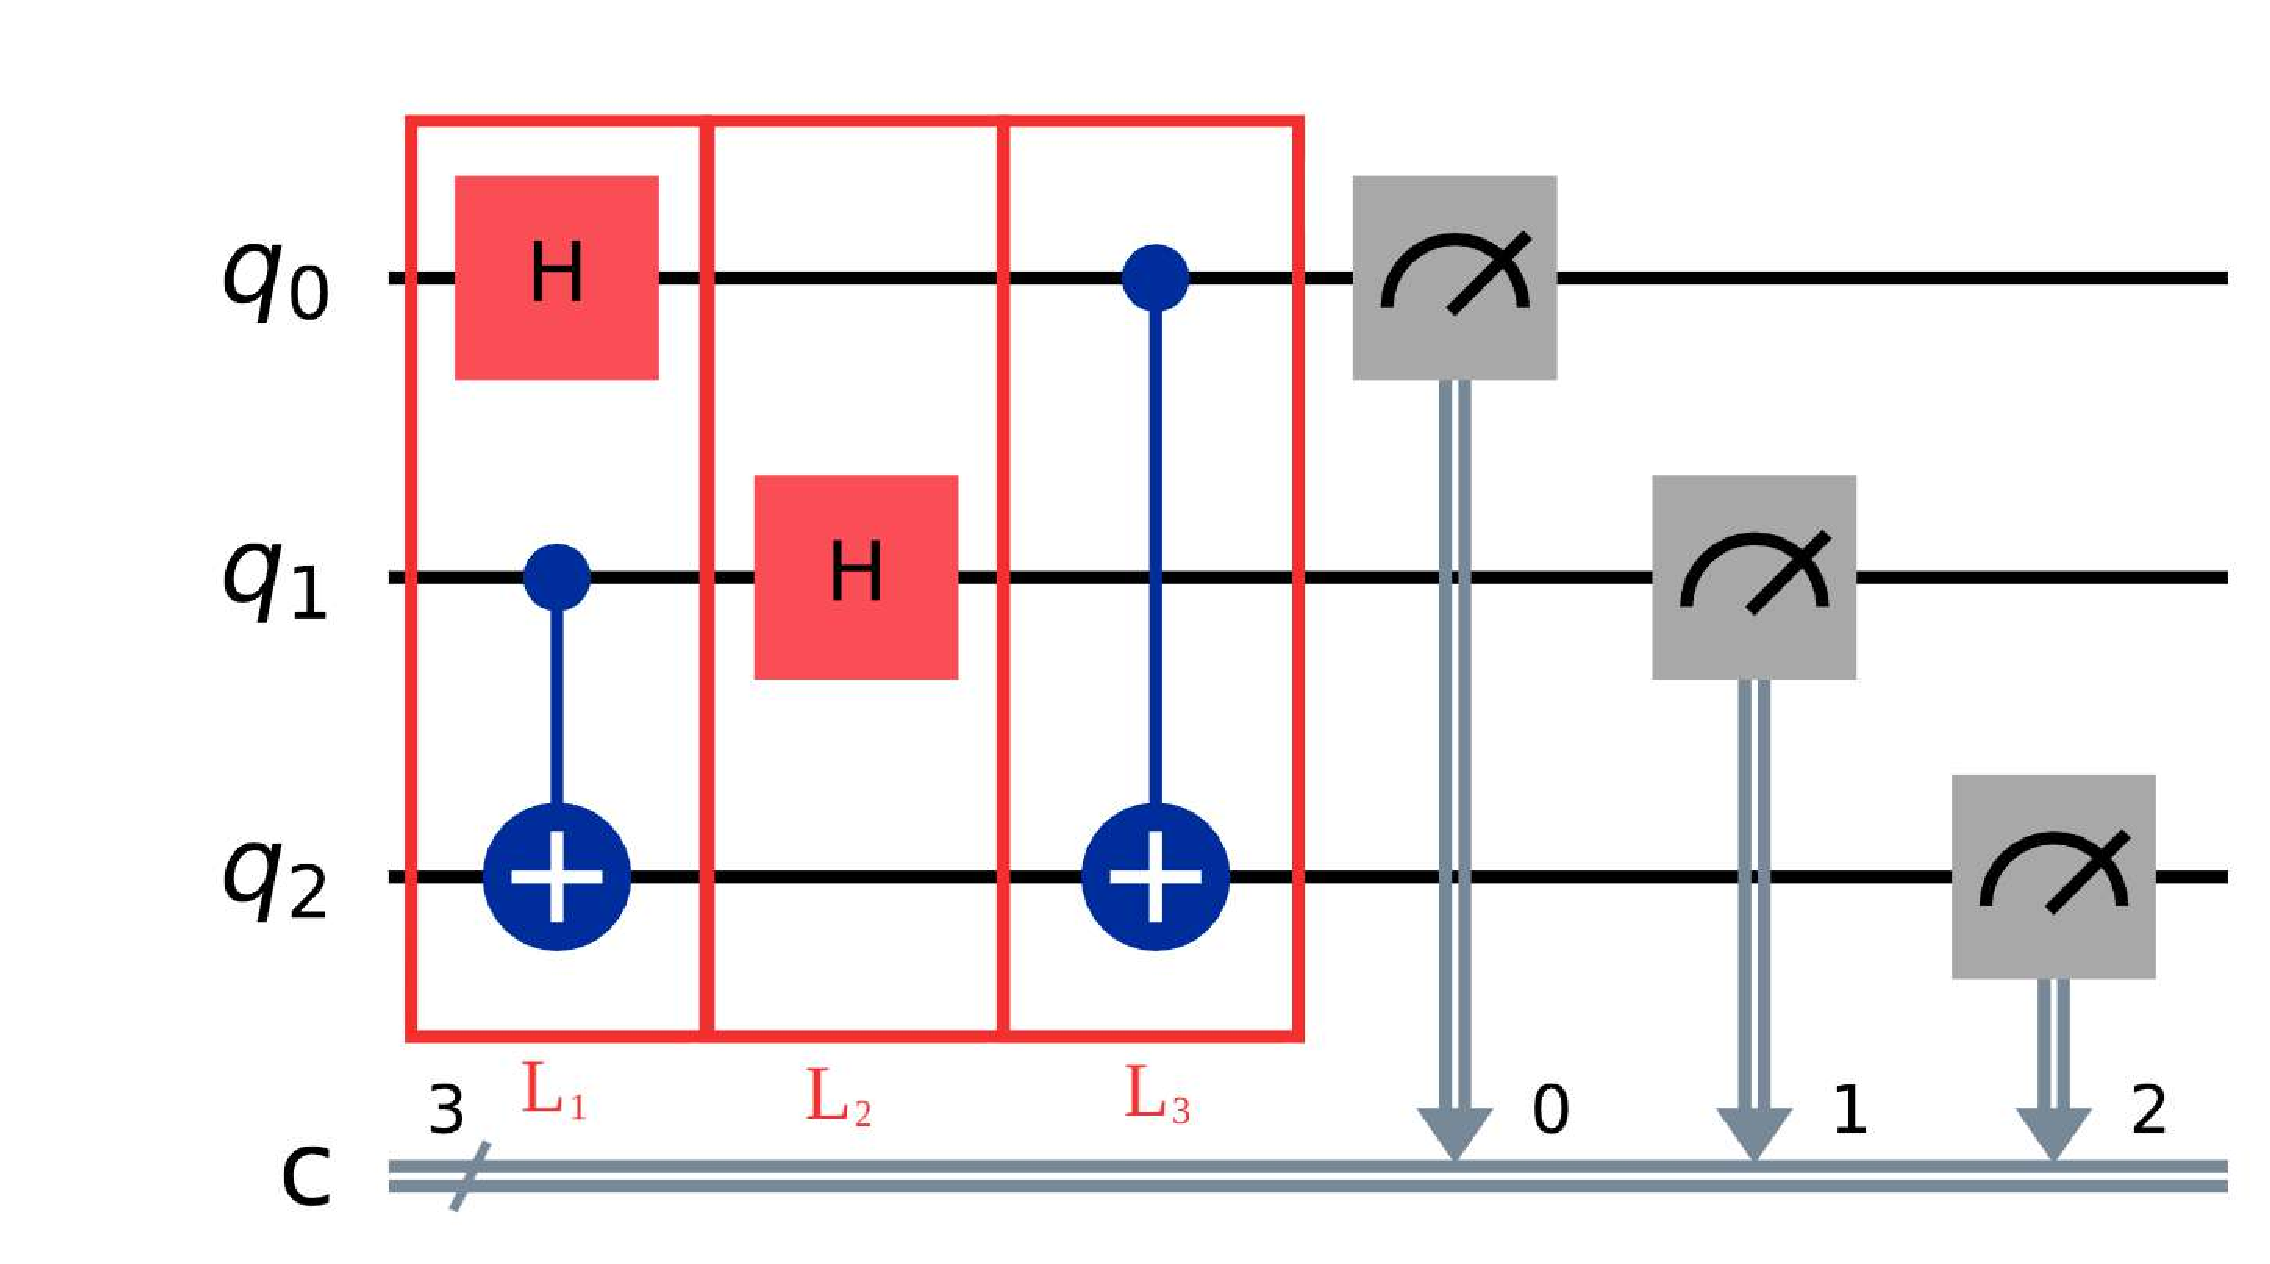
\includegraphics[width=0.5\linewidth]{figures/example_quantum_circuit_with_layers.pdf}
		\caption{The circuit from Figure \ref{fig:example_quantum_circuit} can be split into layers. In every layer, a maximum of one gate act on each qubit.}
		\label{fig:example_quantum_circuit_with_layers}
	\end{figure}
	As shown in Figure \ref{fig:example_quantum_circuit_with_layers}, the circuit can be divided into three layers $L_1$, $L_2$ and $L_3$. Each layer can be imagined as an Unitary operator acting on the composite state of all qubits. The final state $\ket{\psi_{final}}$ can then be determined by applying all operators corresponding to the layers of the circuit to the initial state $\ket{\psi_{initial}}$,
	\begin{equation}
		\label{eq:apply_layers_to_initial_state}
		\ket{\psi_{final}}=\hat{L}_3\hat{L}_2\hat{L}_1\ket{\psi_{initial}}.
	\end{equation}
	To determine the matrix representation of the layers, the matrix representation in the basis $\mathcal{B}$ for each single-qubit gate $U_{(i)}$ and two-qubit gate $U_{(i, j)}$ contained in the layer has to be found. In this notation $i$ and $j$ denote the number of the qubit on which the gate acts, while demanding $i < j$.
	As single-qubit gates leave other qubits untouched, their matrix representation in a basis $\mathcal{B}_N$ for $N$ qubits can be constructed by tensor-products with the identity matrix:
	\begin{equation}
		\label{eq:single_qubit_gate_product_basis}
		U^{\{\mathcal{B}_N\}}_{(i)}=\mathbbm{1}^{\otimes i}\otimes U_{(i)}\otimes \mathbbm{1}^{\otimes N-1-i}
	\end{equation}
	Entangling gates cannot be seperated into single-qubit gates as discussed in Section \ref{sec:multi_qubit_gates}, so to find the matrix representation of entangling gates $U_{(i,j)}$ in the basis $\mathcal{B}_N$ while only knowing the matrix representation of $U_{(i,i+1)}$, a permutation matrix $P$, more specifically a transposition matrix $P_{n\mapsto m}$, has to be applied for entangling gates of non-adjacent qubits that swaps two qubits in a way that qubit $q_i$ and $q_j$ are adjacent,
	\begin{equation}
		\label{eq:qubit_swap}
		q_j\leftrightarrow q_{i+1}
	\end{equation}
	leading to
	\begin{equation}
		\label{eq:two_qubit_gate_product_basis}
		U^{\{\mathcal{B}_N\}}_{(i, j)}=P^{-1}_{i+1\mapsto j}\left(\mathbbm{1}^{\otimes i}\otimes U_{(i,i+1)}\otimes \mathbbm{1}^{\otimes N-2-i}\right)P_{i+1\mapsto j}.
	\end{equation}
	\\
	Coming back to the example from figure \ref{fig:example_quantum_circuit_with_layers} the first layer $L_1$, a Hadamard gate acts on the qubit $q_0$ and a controlled-X gate acts on $q_1$ and $q_2$ where $q_1$ is the control qubit and $q_2$ is the target qubit. Using equations (\ref{eq:single_qubit_gate_product_basis}) and (\ref{eq:two_qubit_gate_product_basis}), $L_1$ can be calculated,
	\begin{equation}
		\label{eq:example_circuit_layer1}
		L_1=\left(H\otimes \mathbbm{1}\otimes \mathbbm{1}\right)\left(\mathbbm{1}\otimes CX\right)=H\otimes CX,
	\end{equation}
	while the permutation matrix $P=\mathbbm{1}$ for $L_1$  as $q_1$ and $q_2$ are already adjacent.
	$L_2$ can be found in a similar fashion as in this layer only a single-qubit Hadamard gate is present:
	\begin{equation}
		\label{eq:example_circuit_layer2}
		L_2=\mathbbm{1}\otimes H\otimes\mathbbm{1}.
	\end{equation}
	In $L_3$ only a controlled-X gate is present. But the qubits it acts on are not adjacent. To make them adjacent a transposition matrix $P_{1\mapsto 2}$ is used. This transposition matrix swaps qubit $q_1$ and $q_2$, so qubit $q_0$ is adjacent to $q_2$. When these qubits are swapped, the basis state order changes. This yields the conditions to determine the permutation matrix:
	\begin{equation}
		\label{eq:example_circuit_permutation_matrix}
		\begin{split}
			P_{1\mapsto 2}\ket{000}&=\ket{000} \\
			P_{1\mapsto 2}\ket{001}&=\ket{010} \\
			P_{1\mapsto 2}\ket{010}&=\ket{001} \\
			P_{1\mapsto 2}\ket{011}&=\ket{011} \\
			P_{1\mapsto 2}\ket{100}&=\ket{100} \\
			P_{1\mapsto 2}\ket{101}&=\ket{110} \\
			P_{1\mapsto 2}\ket{110}&=\ket{101} \\
			P_{1\mapsto 2}\ket{111}&=\ket{111}
		\end{split} \Rightarrow P_{1\mapsto 2}=
		\begin{pmatrix}
			1 & 0 & 0 & 0 & 0 & 0 & 0 & 0 \\
			0 & 0 & 1 & 0 & 0 & 0 & 0 & 0 \\
			0 & 1 & 0 & 0 & 0 & 0 & 0 & 0 \\
			0 & 0 & 0 & 1 & 0 & 0 & 0 & 0 \\
			0 & 0 & 0 & 0 & 1 & 0 & 0 & 0 \\
			0 & 0 & 0 & 0 & 0 & 0 & 1 & 0 \\
			0 & 0 & 0 & 0 & 0 & 1 & 0 & 0 \\
			0 & 0 & 0 & 0 & 0 & 0 & 0 & 1 
		\end{pmatrix}.
	\end{equation}
	$L_3$ can then be determined by using equation (\ref{eq:two_qubit_gate_product_basis}):
	\begin{equation}
		\label{eq:example_circuit_layer3}
		L_3=P^{-1}_{1\mapsto 2}\left(CX\otimes \mathbbm{1}\right)P_{1\mapsto 2}.
	\end{equation}
	Combining all layers yields the circuit Unitary $C$
	\begin{equation}
		\label{eq:example_circuit_unitary}
		C=L_3L_2L_1=\frac{1}{2}
		\begin{pmatrix}
			1 & 1 & 0 & 0 & 1 & 1 & 0 & 0 \\
			0 & 0 & 1 & 1 & 0 & 0 & -1 & -1 \\
			1 & -1 & 0 & 0 & 1 & -1 & 0 & 0 \\
			0 & 0 & -1 & 1 & 0 & 0 & 1 & -1 \\
			0 & 0 & 1 & 1 & 0 & 0 & 1 & 1 \\
			1 & 1 & 0 & 0 & -1 & -1 & 0 & 0 \\
			0 & 0 & -1 & 1 & 0 & 0 & -1 & 1 \\
			1 & -1 & 0 & 0 & -1 & 1 & 0 & 0
		\end{pmatrix}.
	\end{equation}
	By applying $C$ to the initial circuit state $\ket{\psi_{intial}}=\ket{000}$ the final state $\ket{\psi_{final}}$,
	\begin{equation}
		\label{eq:example_circuit_final_state}
		\ket{\psi_{final}}=C\ket{000}=\frac{1}{2}\left(\ket{000}+\ket{010}+\ket{101}+\ket{111}\right)
	\end{equation}
	is computed and the probabilities of measuring each eigenstate can be calculated using equation (\ref{eq:measurement_probability_a}):
	\begin{equation}
		\label{eq:example_circuit_probability_000}
		\abs{\braket{000}{\psi_{final}}}^2=\tfrac{1}{4},
	\end{equation}
	\begin{equation}
		\label{eq:example_circuit_probability_001}
		\abs{\braket{001}{\psi_{final}}}^2=0,
	\end{equation}
	\begin{equation}
		\label{eq:example_circuit_probability_010}
		\abs{\braket{010}{\psi_{final}}}^2=\tfrac{1}{4},
	\end{equation}
	\begin{equation}
		\label{eq:example_circuit_probability_011}
		\abs{\braket{011}{\psi_{final}}}^2=0,
	\end{equation}
	\begin{equation}
		\label{eq:example_circuit_probability_100}
		\abs{\braket{100}{\psi_{final}}}^2=0,
	\end{equation}
	\begin{equation}
		\label{eq:example_circuit_probability_101}
		\abs{\braket{101}{\psi_{final}}}^2=\tfrac{1}{4},
	\end{equation}
	\begin{equation}
		\label{eq:example_circuit_probability_110}
		\abs{\braket{110}{\psi_{final}}}^2=0,
	\end{equation}
	\begin{equation}
		\label{eq:example_circuit_probability_111}
		\abs{\braket{111}{\psi_{final}}}^2=\tfrac{1}{4}.
	\end{equation}
	And indeed, when simulating the circuit with qiskits Aer-Simulator \cite{qiskit2024} with $100000$ runs, the same results are achieved, as seen in Figure \ref{fig:example_circuit_results}.
	\begin{figure}[H]
		\centering
		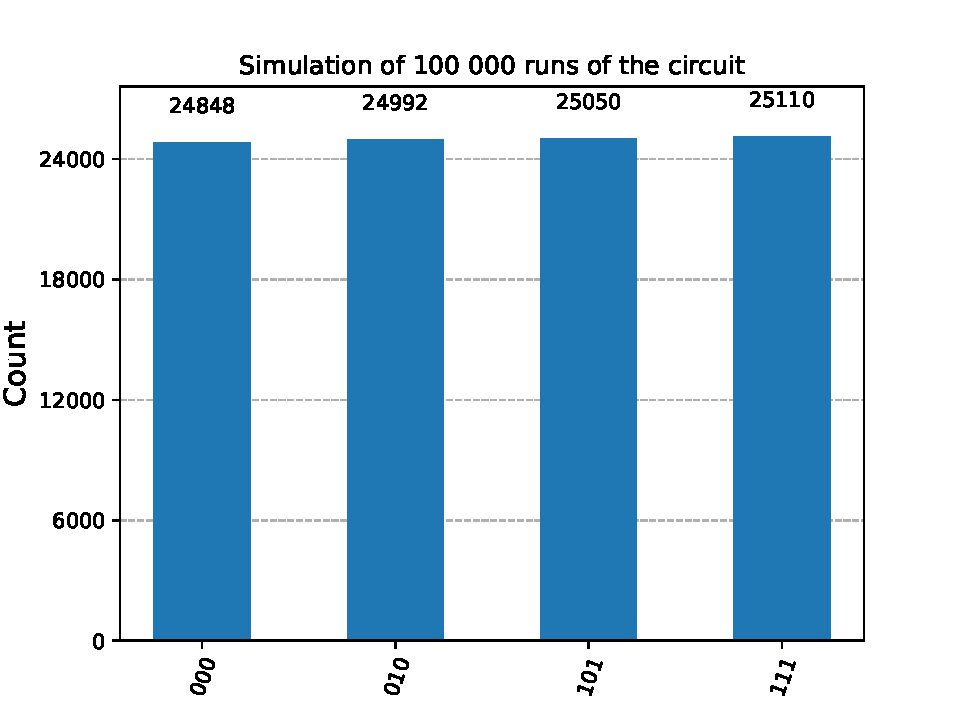
\includegraphics[width=0.7\linewidth]{figures/qc_results.pdf}
		\caption{This plot shows the outcome of a simulation of the circuit from Figure \ref{fig:example_quantum_circuit}. While the states $\ket{000}$, $\ket{010}$, $\ket{101}$ and $\ket{111}$ all have a probability close to $\frac{1}{4}$, the states $\ket{001}$, $\ket{011}$, $\ket{100}$ and $\ket{110}$ are not realized. This coincides with the exact result from equation (\ref{eq:example_circuit_final_state}). This plot was generated using Qiskit \cite{qiskit2024}. The source code for this figure can be found in Listing \ref{lst:circuit_results_source}}
		\label{fig:example_circuit_results}
	\end{figure}

\section{Universal gate sets} \label{sec:universal_gateset}
	The term \textit{Universal Gate Set} is usually defined as follows:
	\begin{definitionbox}
		\textit{A universal gate set is a finite set of gates that can be combined to approximate any Unitary operation on any number of qubits to arbitrary precision.} \cite{Nielsen2010-xd}
	\end{definitionbox}
	It is possible to check if a set of gates is universal by using group-theory methods \cite{Sawicki_2017} or by examining its relation to Unitary t-designs \cite{Sawicki_2022}. One example for a universal gate set that is commonly used is the Clifford + T set \cite{vandaele2024optimal}. It consists of the Hadamard gate $H$ (\ref{eq:hadamard_matrix}), the phase gate $S$ (\ref{eq:s_gate}), the $T$-gate (\ref{eq:t_gate}) and the $CX$ gate (\ref{eq:cx_matrix_representation}). 
	\begin{equation}
		\label{eq:s_gate}
		S=
		\begin{pmatrix}
			1 & 0 \\
			0 & i
		\end{pmatrix}
	\end{equation}
	\begin{equation}
		\label{eq:t_gate}
		T=
		\begin{pmatrix}
			1 & 0 \\
			0 & e^{i\frac{\pi}{4}}
		\end{pmatrix}
	\end{equation}
	By removing the restriction that the set of gates must be finite, the definition becomes simpler:
	\begin{definitionbox}
		\begin{definition}
			\label{def:universal_gate_set}
			A universal gate set is a set of gates that can be combined to produce any Unitary operation on any number of qubits.
		\end{definition}
	\end{definitionbox}
	This definition excludes finite sets of gates, as there are infinetly many Unitary operations. While this definition may not be applicable to real-world scenarios, it is sufficient for this thesis and is therefore used instead of the usual definition.
	One example for a universal gate set that complies with this definition is a set of single-qubit rotations (\ref{eq:u_gate}) in conjunction with the $CZ$-gate,
	\begin{equation}
		\label{eq:cz_gate}
		CZ=
		\begin{pmatrix}
			1 & 0 & 0 & 0 \\
			0 & 1 & 0 & 0 \\
			0 & 0 & 1 & 0 \\
			0 & 0 & 0 & -1 \\
		\end{pmatrix}
	\end{equation}
	Any set of single-qubit gates that is universal for $SU\left(2\right)$, combined with the $CX$-gate (\ref{eq:cx_matrix_representation}) forms a universal gate set \cite{Nielsen2010-xd}. As single-qubit rotations $U\left(\theta,\phi,\lambda\right)$ are universal for $SU\left(2\right)$ by definition and the $CZ$-gate can be constructed using a $CX$ gate and two Hadamard gates,
	\begin{equation}
		\label{eq:cz_construction_with_cx}
		CZ=\left(\mathbbm{1}\otimes H\right)CX\left(\mathbbm{1}\otimes H\right),
	\end{equation}
	the gate set $\{U\left(\theta,\phi,\lambda\right),CZ\}$ is also universal.
	This gate set is later used in this thesis to construct circuits to test circuit compression on.